% Created by tikzDevice version 0.10.1 on 2018-01-31 11:59:41
% !TEX encoding = UTF-8 Unicode
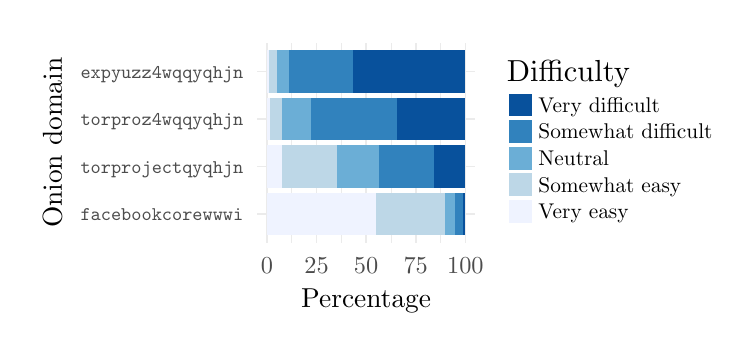
\begin{tikzpicture}[x=1pt,y=1pt]
\definecolor{fillColor}{RGB}{255,255,255}
\path[use as bounding box,fill=fillColor,fill opacity=0.00] (0,0) rectangle (252.94,108.41);
\begin{scope}
\path[clip] ( 82.86, 30.77) rectangle (161.75,102.91);
\definecolor{drawColor}{gray}{0.92}

\path[draw=drawColor,line width= 0.3pt,line join=round] ( 95.41, 30.77) --
	( 95.41,102.91);

\path[draw=drawColor,line width= 0.3pt,line join=round] (113.34, 30.77) --
	(113.34,102.91);

\path[draw=drawColor,line width= 0.3pt,line join=round] (131.27, 30.77) --
	(131.27,102.91);

\path[draw=drawColor,line width= 0.3pt,line join=round] (149.20, 30.77) --
	(149.20,102.91);

\path[draw=drawColor,line width= 0.6pt,line join=round] ( 82.86, 41.08) --
	(161.75, 41.08);

\path[draw=drawColor,line width= 0.6pt,line join=round] ( 82.86, 58.25) --
	(161.75, 58.25);

\path[draw=drawColor,line width= 0.6pt,line join=round] ( 82.86, 75.43) --
	(161.75, 75.43);

\path[draw=drawColor,line width= 0.6pt,line join=round] ( 82.86, 92.60) --
	(161.75, 92.60);

\path[draw=drawColor,line width= 0.6pt,line join=round] ( 86.45, 30.77) --
	( 86.45,102.91);

\path[draw=drawColor,line width= 0.6pt,line join=round] (104.38, 30.77) --
	(104.38,102.91);

\path[draw=drawColor,line width= 0.6pt,line join=round] (122.30, 30.77) --
	(122.30,102.91);

\path[draw=drawColor,line width= 0.6pt,line join=round] (140.23, 30.77) --
	(140.23,102.91);

\path[draw=drawColor,line width= 0.6pt,line join=round] (158.16, 30.77) --
	(158.16,102.91);
\definecolor{fillColor}{RGB}{239,243,255}

\path[fill=fillColor] ( 86.45, 33.35) rectangle (125.91, 48.81);
\definecolor{fillColor}{RGB}{189,215,231}

\path[fill=fillColor] (125.91, 33.35) rectangle (150.65, 48.81);
\definecolor{fillColor}{RGB}{107,174,214}

\path[fill=fillColor] (150.65, 33.35) rectangle (154.48, 48.81);
\definecolor{fillColor}{RGB}{49,130,189}

\path[fill=fillColor] (154.48, 33.35) rectangle (157.43, 48.81);
\definecolor{fillColor}{RGB}{8,81,156}

\path[fill=fillColor] (157.43, 33.35) rectangle (158.17, 48.81);
\definecolor{fillColor}{RGB}{239,243,255}

\path[fill=fillColor] ( 86.45, 50.52) rectangle ( 91.75, 65.98);
\definecolor{fillColor}{RGB}{189,215,231}

\path[fill=fillColor] ( 91.75, 50.52) rectangle (111.78, 65.98);
\definecolor{fillColor}{RGB}{107,174,214}

\path[fill=fillColor] (111.78, 50.52) rectangle (127.09, 65.98);
\definecolor{fillColor}{RGB}{49,130,189}

\path[fill=fillColor] (127.09, 50.52) rectangle (146.68, 65.98);
\definecolor{fillColor}{RGB}{8,81,156}

\path[fill=fillColor] (146.68, 50.52) rectangle (158.17, 65.98);
\definecolor{fillColor}{RGB}{239,243,255}

\path[fill=fillColor] ( 86.45, 67.70) rectangle ( 87.63, 83.15);
\definecolor{fillColor}{RGB}{189,215,231}

\path[fill=fillColor] ( 87.63, 67.70) rectangle ( 91.91, 83.15);
\definecolor{fillColor}{RGB}{107,174,214}

\path[fill=fillColor] ( 91.91, 67.70) rectangle (102.39, 83.15);
\definecolor{fillColor}{RGB}{49,130,189}

\path[fill=fillColor] (102.39, 67.70) rectangle (133.38, 83.15);
\definecolor{fillColor}{RGB}{8,81,156}

\path[fill=fillColor] (133.38, 67.70) rectangle (158.17, 83.15);
\definecolor{fillColor}{RGB}{239,243,255}

\path[fill=fillColor] ( 86.45, 84.87) rectangle ( 87.34,100.33);
\definecolor{fillColor}{RGB}{189,215,231}

\path[fill=fillColor] ( 87.34, 84.87) rectangle ( 90.15,100.33);
\definecolor{fillColor}{RGB}{107,174,214}

\path[fill=fillColor] ( 90.15, 84.87) rectangle ( 94.31,100.33);
\definecolor{fillColor}{RGB}{49,130,189}

\path[fill=fillColor] ( 94.31, 84.87) rectangle (117.71,100.33);
\definecolor{fillColor}{RGB}{8,81,156}

\path[fill=fillColor] (117.71, 84.87) rectangle (158.16,100.33);
\end{scope}
\begin{scope}
\path[clip] (  0.00,  0.00) rectangle (252.94,108.41);
\definecolor{drawColor}{gray}{0.30}

\node[text=drawColor,anchor=base east,inner sep=0pt, outer sep=0pt, scale=  0.70] at ( 77.91, 38.65) {\texttt{facebookcorewwwi}};

\node[text=drawColor,anchor=base east,inner sep=0pt, outer sep=0pt, scale=  0.70] at ( 77.91, 55.83) {\texttt{torprojectqyqhjn}};

\node[text=drawColor,anchor=base east,inner sep=0pt, outer sep=0pt, scale=  0.70] at ( 77.91, 73.00) {\texttt{torproz4wqqyqhjn}};

\node[text=drawColor,anchor=base east,inner sep=0pt, outer sep=0pt, scale=  0.70] at ( 77.91, 90.18) {\texttt{expyuzz4wqqyqhjn}};
\end{scope}
\begin{scope}
\path[clip] (  0.00,  0.00) rectangle (252.94,108.41);
\definecolor{drawColor}{gray}{0.30}

\node[text=drawColor,anchor=base,inner sep=0pt, outer sep=0pt, scale=  0.88] at ( 86.45, 19.76) {0};

\node[text=drawColor,anchor=base,inner sep=0pt, outer sep=0pt, scale=  0.88] at (104.38, 19.76) {25};

\node[text=drawColor,anchor=base,inner sep=0pt, outer sep=0pt, scale=  0.88] at (122.30, 19.76) {50};

\node[text=drawColor,anchor=base,inner sep=0pt, outer sep=0pt, scale=  0.88] at (140.23, 19.76) {75};

\node[text=drawColor,anchor=base,inner sep=0pt, outer sep=0pt, scale=  0.88] at (158.16, 19.76) {100};
\end{scope}
\begin{scope}
\path[clip] (  0.00,  0.00) rectangle (252.94,108.41);
\definecolor{drawColor}{RGB}{0,0,0}

\node[text=drawColor,anchor=base,inner sep=0pt, outer sep=0pt, scale=  0.99] at (122.31,  7.44) {Percentage};
\end{scope}
\begin{scope}
\path[clip] (  0.00,  0.00) rectangle (252.94,108.41);
\definecolor{drawColor}{RGB}{0,0,0}

\node[text=drawColor,rotate= 90.00,anchor=base,inner sep=0pt, outer sep=0pt, scale=  0.99] at ( 12.32, 66.84) {Onion domain};
\end{scope}
\begin{scope}
\path[clip] (  0.00,  0.00) rectangle (252.94,108.41);
\definecolor{drawColor}{RGB}{0,0,0}

\node[text=drawColor,anchor=base west,inner sep=0pt, outer sep=0pt, scale=  1.10] at (173.13, 88.95) {Difficulty};
\end{scope}
\begin{scope}
\path[clip] (  0.00,  0.00) rectangle (252.94,108.41);
\definecolor{fillColor}{RGB}{8,81,156}

\path[fill=fillColor] (173.85, 76.41) rectangle (182.06, 84.62);
\end{scope}
\begin{scope}
\path[clip] (  0.00,  0.00) rectangle (252.94,108.41);
\definecolor{fillColor}{RGB}{49,130,189}

\path[fill=fillColor] (173.85, 66.77) rectangle (182.06, 74.99);
\end{scope}
\begin{scope}
\path[clip] (  0.00,  0.00) rectangle (252.94,108.41);
\definecolor{fillColor}{RGB}{107,174,214}

\path[fill=fillColor] (173.85, 57.14) rectangle (182.06, 65.35);
\end{scope}
\begin{scope}
\path[clip] (  0.00,  0.00) rectangle (252.94,108.41);
\definecolor{fillColor}{RGB}{189,215,231}

\path[fill=fillColor] (173.85, 47.50) rectangle (182.06, 55.72);
\end{scope}
\begin{scope}
\path[clip] (  0.00,  0.00) rectangle (252.94,108.41);
\definecolor{fillColor}{RGB}{239,243,255}

\path[fill=fillColor] (173.85, 37.87) rectangle (182.06, 46.08);
\end{scope}
\begin{scope}
\path[clip] (  0.00,  0.00) rectangle (252.94,108.41);
\definecolor{drawColor}{RGB}{0,0,0}

\node[text=drawColor,anchor=base west,inner sep=0pt, outer sep=0pt, scale=  0.77] at (184.58, 77.86) {Very difficult};
\end{scope}
\begin{scope}
\path[clip] (  0.00,  0.00) rectangle (252.94,108.41);
\definecolor{drawColor}{RGB}{0,0,0}

\node[text=drawColor,anchor=base west,inner sep=0pt, outer sep=0pt, scale=  0.77] at (184.58, 68.23) {Somewhat difficult};
\end{scope}
\begin{scope}
\path[clip] (  0.00,  0.00) rectangle (252.94,108.41);
\definecolor{drawColor}{RGB}{0,0,0}

\node[text=drawColor,anchor=base west,inner sep=0pt, outer sep=0pt, scale=  0.77] at (184.58, 58.59) {Neutral};
\end{scope}
\begin{scope}
\path[clip] (  0.00,  0.00) rectangle (252.94,108.41);
\definecolor{drawColor}{RGB}{0,0,0}

\node[text=drawColor,anchor=base west,inner sep=0pt, outer sep=0pt, scale=  0.77] at (184.58, 48.96) {Somewhat easy};
\end{scope}
\begin{scope}
\path[clip] (  0.00,  0.00) rectangle (252.94,108.41);
\definecolor{drawColor}{RGB}{0,0,0}

\node[text=drawColor,anchor=base west,inner sep=0pt, outer sep=0pt, scale=  0.77] at (184.58, 39.32) {Very easy};
\end{scope}
\end{tikzpicture}
